\begin{Exercise}[title={Stack},difficulty=5]
\label{ex:stack}
\Question \label{ex:stack q1} Create a simple stack which can hold a
fixed amount of ints. It does not have to grow beyond this limit.
Define both a \func{push} -- put something on the stack -- and a \func{pop} 
-- retrieve something fro the stack -- function. The stack should be
a LIFO (last in, first out) stack.

\begin{figure}[H]
\caption{A simple LIFO stack}
\label{fig:stack}
\begin{center}
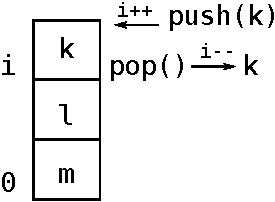
\includegraphics[scale=0.65]{fig/stack.pdf}
\end{center}
\end{figure}

\Question \label{ex:stack q2} Bonus. Write a \func{String} method which 
converts the stack to a string representation.  This way you can print the stack using:
\lstinline{fmt.Printf("My stack %v\n", stack)}

\noindent{}The stack in the figure could be represented as:
\texttt{[0:m] [1:l] [2:k]}

\end{Exercise}

\begin{Answer}

\Question 
%%\subsection*{Define our type} maybe nice to do this
First we define a new type that represents a stack; we need an
array (to hold the keys) and an index, which points to the last element.
Our small stack can only hold 10 elements.

\begin{lstlisting}
type stack struct { |\coderemark{\emph{stack} is not exported}|
    i    int 
    data [10]int  
}
\end{lstlisting}

Next we need the \func{push} and \func{pop} functions to actually
use the thing. \emph{First we show the \emph{wrong}{} solution!}
In Go data passed to functions is \emph{passed-by-value} meaning a copy
is created and given to the function. The first stab for the function
\func{push} could be:

\begin{lstlisting}
func (s stack) push(k int) { |\coderemark{Works on copy of argument}|
	if s.i+1 > 9 {
		return
	}
	s.data[s.i] = k
	s.i++
}
\end{lstlisting}
The function works on the \var{s} which is of the type \type{stack}. To
use this we just call \lstinline{s.push(50)}, to push the integer 50 on
the stack. But the push function gets a copy of \var{s}, so it is
\emph{not} working the \emph{real} thing. Nothing gets pushed to our
stack this way, for example the following code:

\begin{lstlisting}
var s stack |\coderemark{make \var{s} a simple \type{stack} variable}|
s.push(25)
fmt.Printf("stack %v\n", s);
s.push(14)
fmt.Printf("stack %v\n", s);
\end{lstlisting}
prints:
\vskip\baselineskip
\begin{display}
stack [0:0]
stack [0:0]
\end{display}
\vskip\baselineskip

To solve this we need to give the function \func{push} a pointer
to the stack. This means we need to change \func{push} from

\lstinline{func (s stack) push(k int)} 
$\rightarrow$
\lstinline{func (s *stack) push(k int)}

We should now use \func{new()} (see "\titleref{sec:allocation with new}"
in chapter \ref{chap:beyond}) to create a \emph{pointer} to a newly
allocated \type{stack}, so line 1 from the example above needs to be
\lstinline{s := new(stack)}

\noindent{}And our two functions become:

\begin{lstlisting}[caption=The push and pop functions]
func (s *stack) push(k int) {
	s.data[s.i] = k
	s.i++
}

func (s *stack) pop() int {
	s.i--
	return s.data[s.i]
}
\end{lstlisting}

Which we then use as follows

\begin{lstlisting}[caption=Stack usage]
func main() {
	var s stack
	s.push(25)
	s.push(14)
	fmt.Printf("stack %v\n", s)
}
\end{lstlisting}

\Question While this was a bonus question, having the ability to print
the stack was very valuable when writing the code for this exercise.
According to the Go documentation \lstinline{fmt.Printf("%v")} can
print any value (\%v) that satisfies the \func{Stringer} interface.
For this to work we only need to define a \func{String()} function for
our type:
\begin{lstlisting}[caption=stack.String()]
func (s stack) String() string {
	var str string
	for i := 0; i <= s.i; i++ {
		str = str + "[" +
			strconv.Itoa(i) + ":" + strconv.Itoa(s.data[i]) + "]"
	}
	return str
}
\end{lstlisting}
\end{Answer}
